\chapter{Introduction}
\label{sec:Introduction}

{
\begin{flushright}
\textit{"There is one quality more important than know-how [...] This is \\ know-what by which we determine not only how to accomplish our \\  purposes, but what our purposes are to be."} 
\emph{-- Norbert Wiener}
\end{flushright}
}
\vspace{10pt}

%There is one quality more important than know-how.... This is know-how by which we determine not only how to accomplish our purposes, but what our purposes are to be.
%Norbert Wiener

%As an engineer I'm constantly spotting problems and plotting how to solve them. James Dyson

This thesis proposes an actuation technology and control schemes addressing the fundamental problem of efficient power-transmission in diverse situation. In many robotic systems, actuators are often required to operate in distinctively different torque-speed load conditions. Machine tools, for instance, are usually either moving at high-speed unloaded during reaching phases, or moving slowly applying large forces during manufacturing operations (see Fig. \ref{fig:machinetool}). Also a legged robot, for example, has to move its leg forward quickly through the air and, once touching the ground, it has to bear a large load (see Fig. \ref{fig:leggedrobot}), or a gripper needs to reach the part quickly and then has to apply large holding forces (see Fig. \ref{fig:gripper}).
%
\begin{figure}[H]
				\vspace{-10pt}
        \centering
				\subfloat[Machine tool]{
				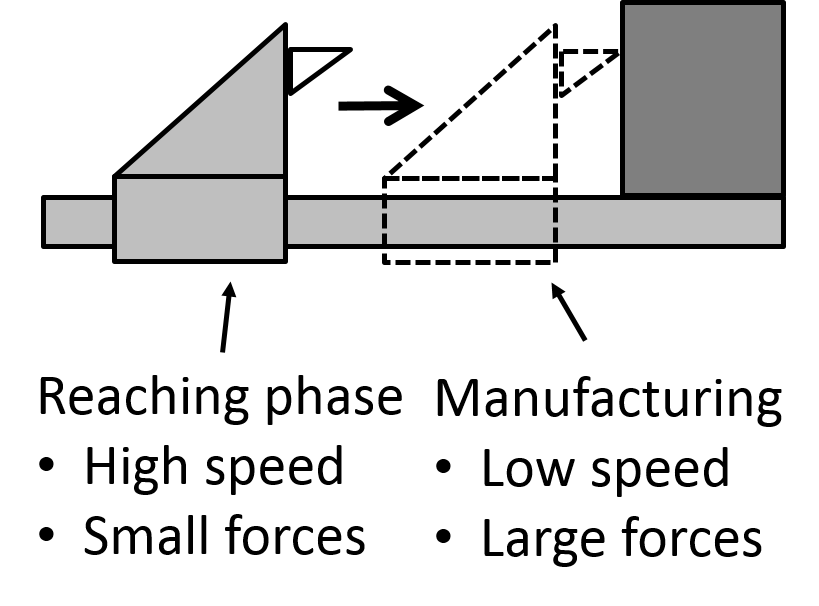
\includegraphics[width=0.30\textwidth]{machinetool.png}
				\label{fig:machinetool}}
        \subfloat[Legged robot]{
				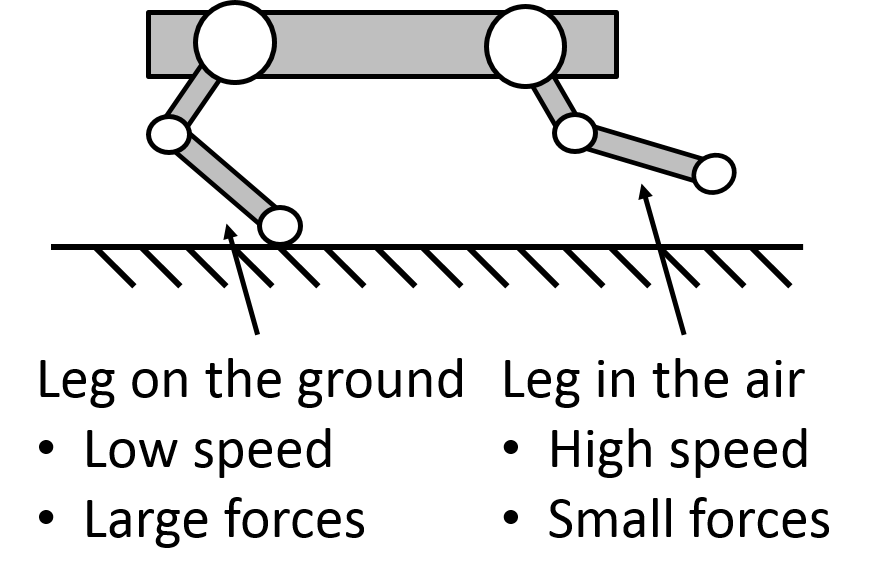
\includegraphics[width=0.30\textwidth]{leggedrobot.png}
				\label{fig:leggedrobot}}
				\subfloat[Gripper]{
				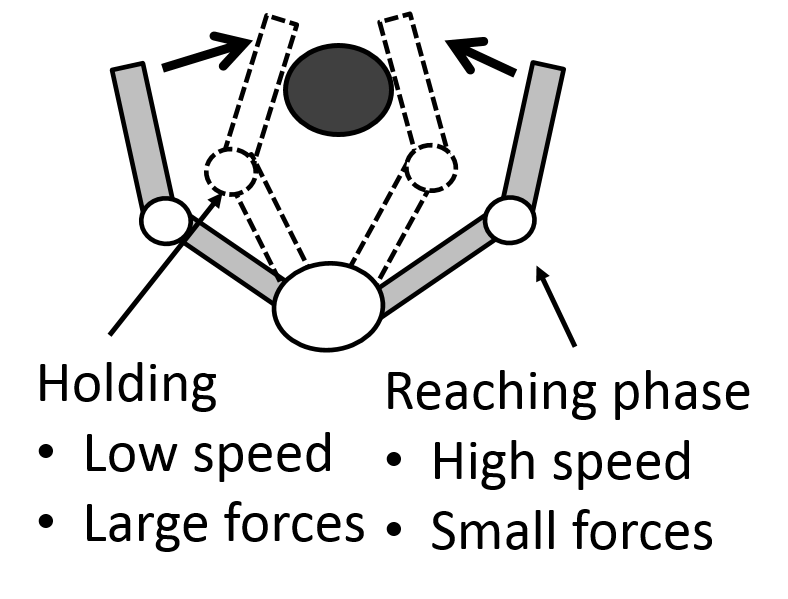
\includegraphics[width=0.30\textwidth]{gripper.png}
				\label{fig:gripper}}
        \caption{Robotics system encountering very different load situation}
				\label{fig:app}
\end{figure}

These two operating conditions, high speed at low torque vs. high torque at low speed, are often an order of magnitude different, while the required output power is similarly low. This discrepancy in requirements is problematic as most actuators will be operating far for their optimal conditions with a gear ratio picked from a middle ground. Electromagnetic actuators are not optimal in term of efficiency and power output at extremum torque-speed conditions. This often leads to the use of over-sized and inefficient actuators, which is inhibitory particularly for mobile robots.


%\section{Limitation of traditional actuation systems}
%\label{sec:limitationOfTraditionnalRoboticSystems}
%
%\paragraph{Electric motors} When compared to other types of actuation technologies or to biological air muscles in the context of human-scale robots, electric motor have relatively goods performances with a power efficiency of about 200 W/Kg, as illustrated at table XXX. However, the power is mostly available at high velocities and a mechanical transmission with a large reduction is usually used. But even when using a reduction ratio, torque-speed characteristic of the motor can be matched to single operating point, and if the motor is required to operate on a wide range of output speed great compromise must be made when selecting the reduction ratio. %Moreover, when a large reduction ratio is used, the actuator intrinsic impedance is too large to make possible a good control of the output force, which is a highly desirable characteristic for interaction tasks.

%actuator table here

%oversize motor figure


\section{Proposed approach: Variable Transmissions}
\label{sec:ProposedSolutionRobotsUsingMultipleGearRatioActuators}


To meet the power requirement of all operating points with small actuators, it is proposed to use electric motors coupled to a gearbox where the gear-ratio can be drastically changed online, see Fig. \ref{fig:2s}. 

\begin{figure}[htb]
        \centering
				\subfloat[two drastically different gear-ratios]{
				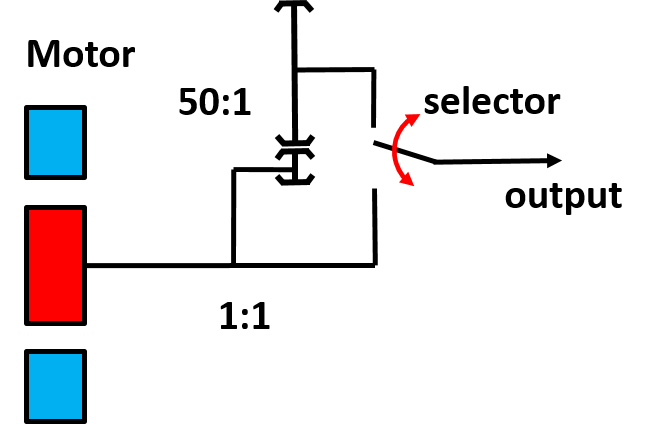
\includegraphics[width=0.40\textwidth]{2speed.png}}
        \subfloat[discrete operating modes]{
				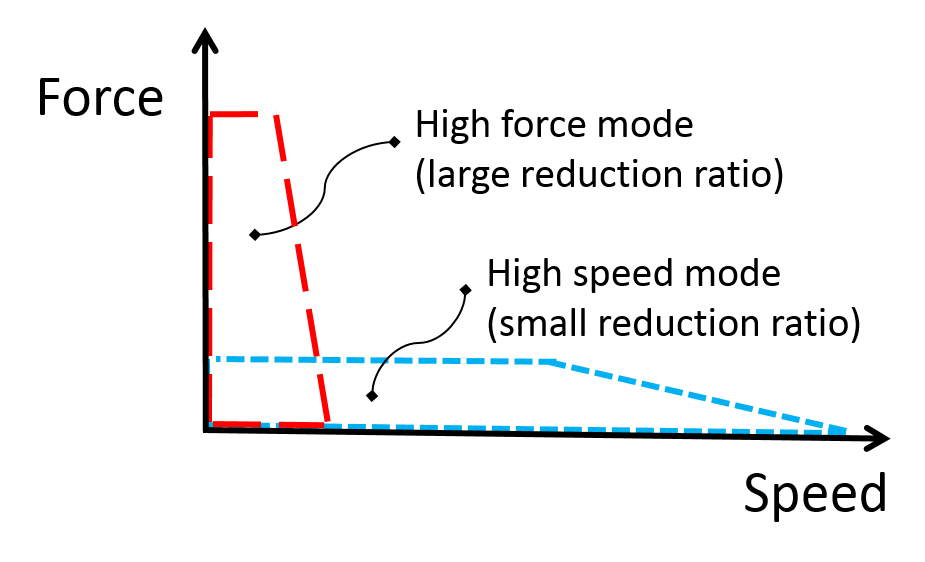
\includegraphics[width=0.45\textwidth]{1DOFmodes.png}}
        \caption{Variable gear-ratio actuator with two discrete options}\label{fig:2s}
\end{figure}


The two main advantage of the approach are: \textbf{good power output and efficiency for a wide range of output speeds} and \textbf{radical changes of intrinsic impedance} (goes with the square of the reduction ratio). 

\subsection{Features of gear-shifting in a robotic context}

\paragraph{Power output and efficiency over a wide range of speed}
In many situation, using multiple gear ratios allows for the downsizing of the motors while still meeting required forces/speeds capabilities. A small lightweight actuator can generate large torques and move at high speed if equipped with both a large and a small gear-ratio. Furthermore, by actively selecting gearing ratios to keep motors in efficient regimes, the energy consumption of a robot can be greatly reduced. 

\paragraph{Radical changes of reflected impedance}
The gear-ratio has a radical effect on the output impedance of a robot; the motor inertia and viscous damping are reflected to the output proportionally with the square of the gearing ratio. Gear-shifting can thus also be used as an alternative approach to variable impedance actuation. A robot joint could be made back-drivable by selecting a small reduction ratio, to interact safely with the environment.  Alternatively, a joint could be made non-backdrivable by selecting a very large reduction ratio to hold a weight without consuming power.

\paragraph{Exploitation or attenuation of the external load dynamics}
Changing the gear-ratio has a radical effect on the natural dynamics of a system. By changing dynamically the gear-ratio, it is possible to select the natural dynamic behavior that is most advantageous for a task. For instance, selecting a small reduction ratio to exploit gravitational forces pulling the robot in a desired direction, or on the other hand, selecting a large reduction ratio to be insensitive to external disturbances.

\paragraph{Directionality of properties}
For a multiple DoF mechanism, the speed/force properties are directional. Typically the Jacobian of a mechanism is only a function of the configuration $J=J(\vec{q})$, but a mechanism using $m$ variable gear-ratio actuators with $n$ possible gear-ratio, the Jacobian (from actuator coordinates to task-space coordinates) would also be function of the gear-ratios selected, i.e. dependent on control inputs $\vec{u}$ : $J=J(\vec{q},\vec{u})$. Hence, for a given configuration there is $n^m$ manipulability ellipsoid option. Fig. \ref{fig:gearselectionlegged} illustrates situations where gear-ratios would be picked to meet the task requirement.


\begin{figure}[H]
	\centering
		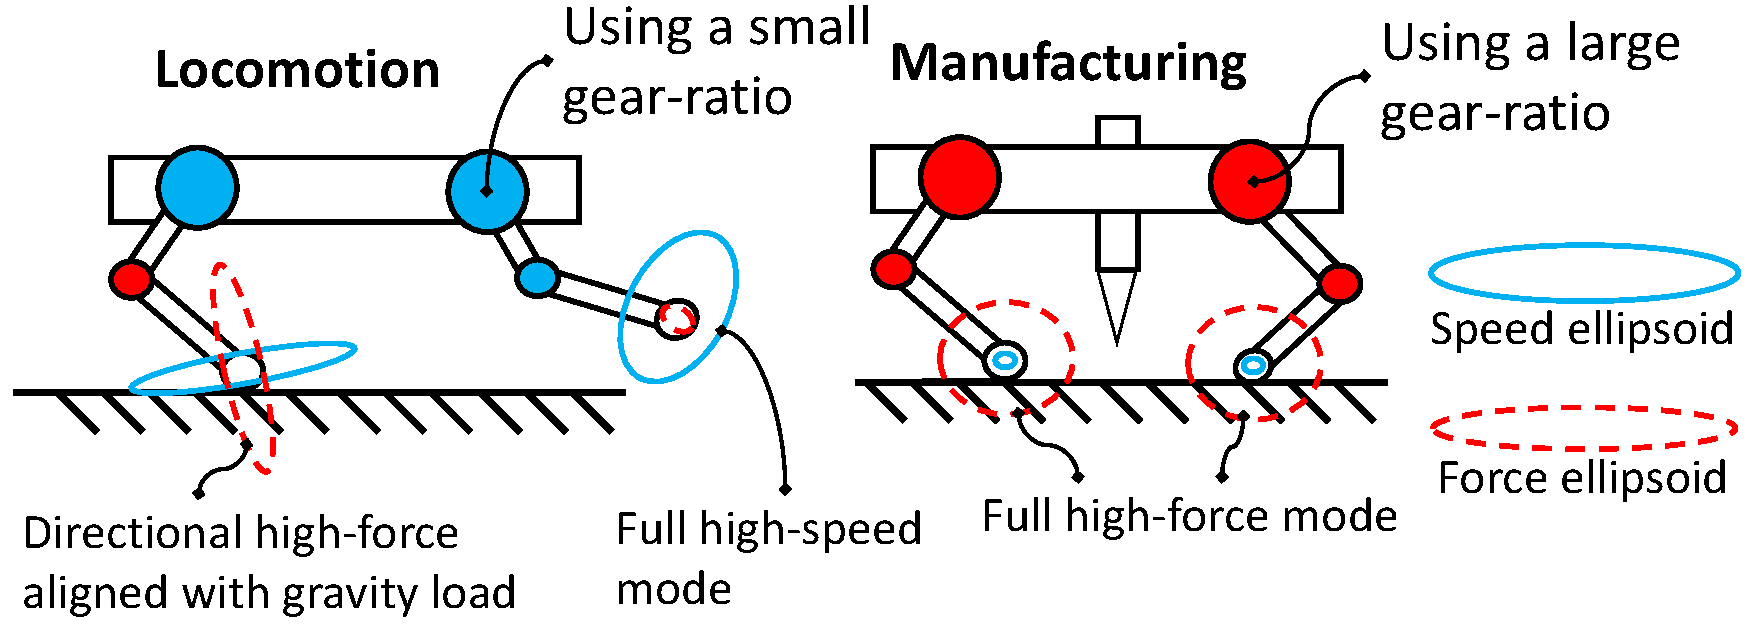
\includegraphics[width=0.80\textwidth]{gearselectionlegged.pdf}
	\caption{Example of advantageous gear selection with a multi-DOF robot}
	\label{fig:gearselectionlegged}
\end{figure}


\section{Main challenges}
\label{sec:MainChallenges}

\paragraph{How to make fast and seamless gearshift?}
Gear shifting is more technically challenging in robotics applications than in vehicle applications. For powertrains, the load is mostly a large inertia, while for robots, the loads may exhibit a rich range of dynamics including spring-like and damper-like loads. Hence, unlike vehicle applications, leaving the load free momentarily during transitions (from one gear-ratio to another) is not acceptable in the context of robotics. Moreover, many robotic applications would benefit from having order-of-magnitudes difference between the possible gear-ratios, i.e. a wider range of ratio than what is typical in vehicle power-train. Hence, an effective gear shifting methodology adapted to robotics is needed, allowing for fast and seamless transitions between very different gear-ratios under diverse load conditions.

\paragraph{When to use what gear-ratio?}
From the control perspective, automating the gear-ratio selection in a robotic context is a new and challenging problem. Gear-shifting is a very non-linear process and the plant becomes a hybrid dynamical system if the usable gear-ratios are a set of discrete values. Hence, no classical control approach can be applied directly to handle the additional gear-ratio selection control input. In simple scenarios, the gear-ratio selection can be based on simple principles. However, to handle the generalize problem of the gear-ratio selection for multi-DoF robots, that experience diverse types of forces acting simultaneously and coupling between each axis, new methodologies are needed to generate trajectories and feedback laws that would use effectively all the gear-ratios options and exploit their advantages.



\section{Original contributions}
\label{sec:contribution}

The two main contributions of this thesis are the development of a \emph{\textbf{gear-shifting methodology adapted to robotics}}, and \emph{\textbf{control algorithms to select dynamically the optimal gear-ratios}}. Also, to the knowledge of the author, the work in this thesis is the first exploration of closed-loop selection of gear-ratios for multi-DoF robotic systems. 


\subsection{Gear-shifting methodology adapted to robotics}

The first contribution of the thesis is an actuation technology capable of fast and seamless gear-shift between two discrete order-of-magnitude different gear-ratios. This technology consist of a mechanical architecture, that will be refer as DSDM (dual-speed dual-motor), used in conjunction with novel gear-shifting control algorithms. The key idea is exploiting the internal degree-of-freedom (DoF) of the actuator to make possible transiting for one gear-ratio to another while also always fully controlling the output load. 

\subsection{Control algorithms to select gear-ratios dynamically}

The second major contribution of this thesis, is the development of intelligent automatic gear-ratio selection schemes for robotic systems. A closed-from solution for the optimal gear-ratios of an arbitrary $n$-DoF robotic system along a known trajectory is derived. Control laws extending this principle to online optimal gear-ratios selection based on state feedback are then developed. The key idea is to used a model to estimate intrinsic and extrinsic forces, to compute if it is more advantageous to attenuate extrinsic forces with large gear-ratios or alternatively to leverage them with a small gear-ratios. The method can be applied to arbitrary $n$-DoF non-linear robotic systems, using actuator with any kind of variable gear-reducer. Moreover, a robust version of the control algorithm that can use some knowledge about the level of uncertainty to improve the gear-ratio selection decision is also developed.


\section{Main results}
\label{sec:mainresults}



\subsection{Prototypes}


\subsection{Theoretical}


\subsection{Simulations}


\subsection{Experiments}




\section{Organization of the thesis}
\label{sec:OrganisationOfTheThesis}

First, chapter \ref{sec:VisionForAircraftManufacturingAutomation} discuss manufacturing applications that would benefict from the developped technologies in this thesis. Chapter \ref{sec:MultipleSpeedActuationTechnology} then present a variable gear-ratio actuator technology using a gear-shifting methodology adapted to robotics. Chapter \ref{sec:ControlAndPlanningOfRobotUsingVariableGearRatioActuators} explore the generalized problem of dynamic selection of gear-ratios for a robotic systems equipped with variable gear-reducer, and present control algorithms. Chapter \ref{sec:ExperimentalValidation} present the prototype robotic system that is used in all experiments throughout the thesis and discuss the mechanical design and the control system implementation. Chapter \ref{sec:casestudy} presents examples of using the proposed control algorithms in different situations.


